\documentclass[]{tufte-handout}

% ams
\usepackage{amssymb,amsmath}

\usepackage{ifxetex,ifluatex}
\usepackage{fixltx2e} % provides \textsubscript
\ifnum 0\ifxetex 1\fi\ifluatex 1\fi=0 % if pdftex
  \usepackage[T1]{fontenc}
  \usepackage[utf8]{inputenc}
\else % if luatex or xelatex
  \makeatletter
  \@ifpackageloaded{fontspec}{}{\usepackage{fontspec}}
  \makeatother
  \defaultfontfeatures{Ligatures=TeX,Scale=MatchLowercase}
  \makeatletter
  \@ifpackageloaded{soul}{
     \renewcommand\allcapsspacing[1]{{\addfontfeature{LetterSpace=15}#1}}
     \renewcommand\smallcapsspacing[1]{{\addfontfeature{LetterSpace=10}#1}}
   }{}
  \makeatother

\fi

% graphix
\usepackage{graphicx}
\setkeys{Gin}{width=\linewidth,totalheight=\textheight,keepaspectratio}

% booktabs
\usepackage{booktabs}

% url
\usepackage{url}

% hyperref
\usepackage{hyperref}

% units.
\usepackage{units}


\setcounter{secnumdepth}{2}

% citations

% pandoc syntax highlighting

% longtable
\usepackage{longtable,booktabs}

% multiplecol
\usepackage{multicol}

% strikeout
\usepackage[normalem]{ulem}

% morefloats
\usepackage{morefloats}


% tightlist macro required by pandoc >= 1.14
\providecommand{\tightlist}{%
  \setlength{\itemsep}{0pt}\setlength{\parskip}{0pt}}

% title / author / date
\title{TP2 - Reconocimiento de Patrones}
\author{Elio Campitelli}
\date{}

\usepackage{booktabs}
\usepackage{longtable}
\usepackage{array}
\usepackage{multirow}
\usepackage{wrapfig}
\usepackage{float}
\usepackage{colortbl}
\usepackage{pdflscape}
\usepackage{tabu}
\usepackage{threeparttable}
\usepackage{threeparttablex}
\usepackage[normalem]{ulem}
\usepackage{makecell}
\usepackage{xcolor}

\begin{document}

\maketitle




\hypertarget{datos}{%
\section{Datos}\label{datos}}

En este TP voy a estar usando la base de datos \texttt{penguins} del paquete de R \textbf{palmerpenguins} (KB, TD, and WR 2014). Los datos recolectados por la Dra. Kristen Gorman en la Estación Palmer, consisten en mediciones de la longitud del culmen\footnote{El culmen es la parte superior del pico de las aves. 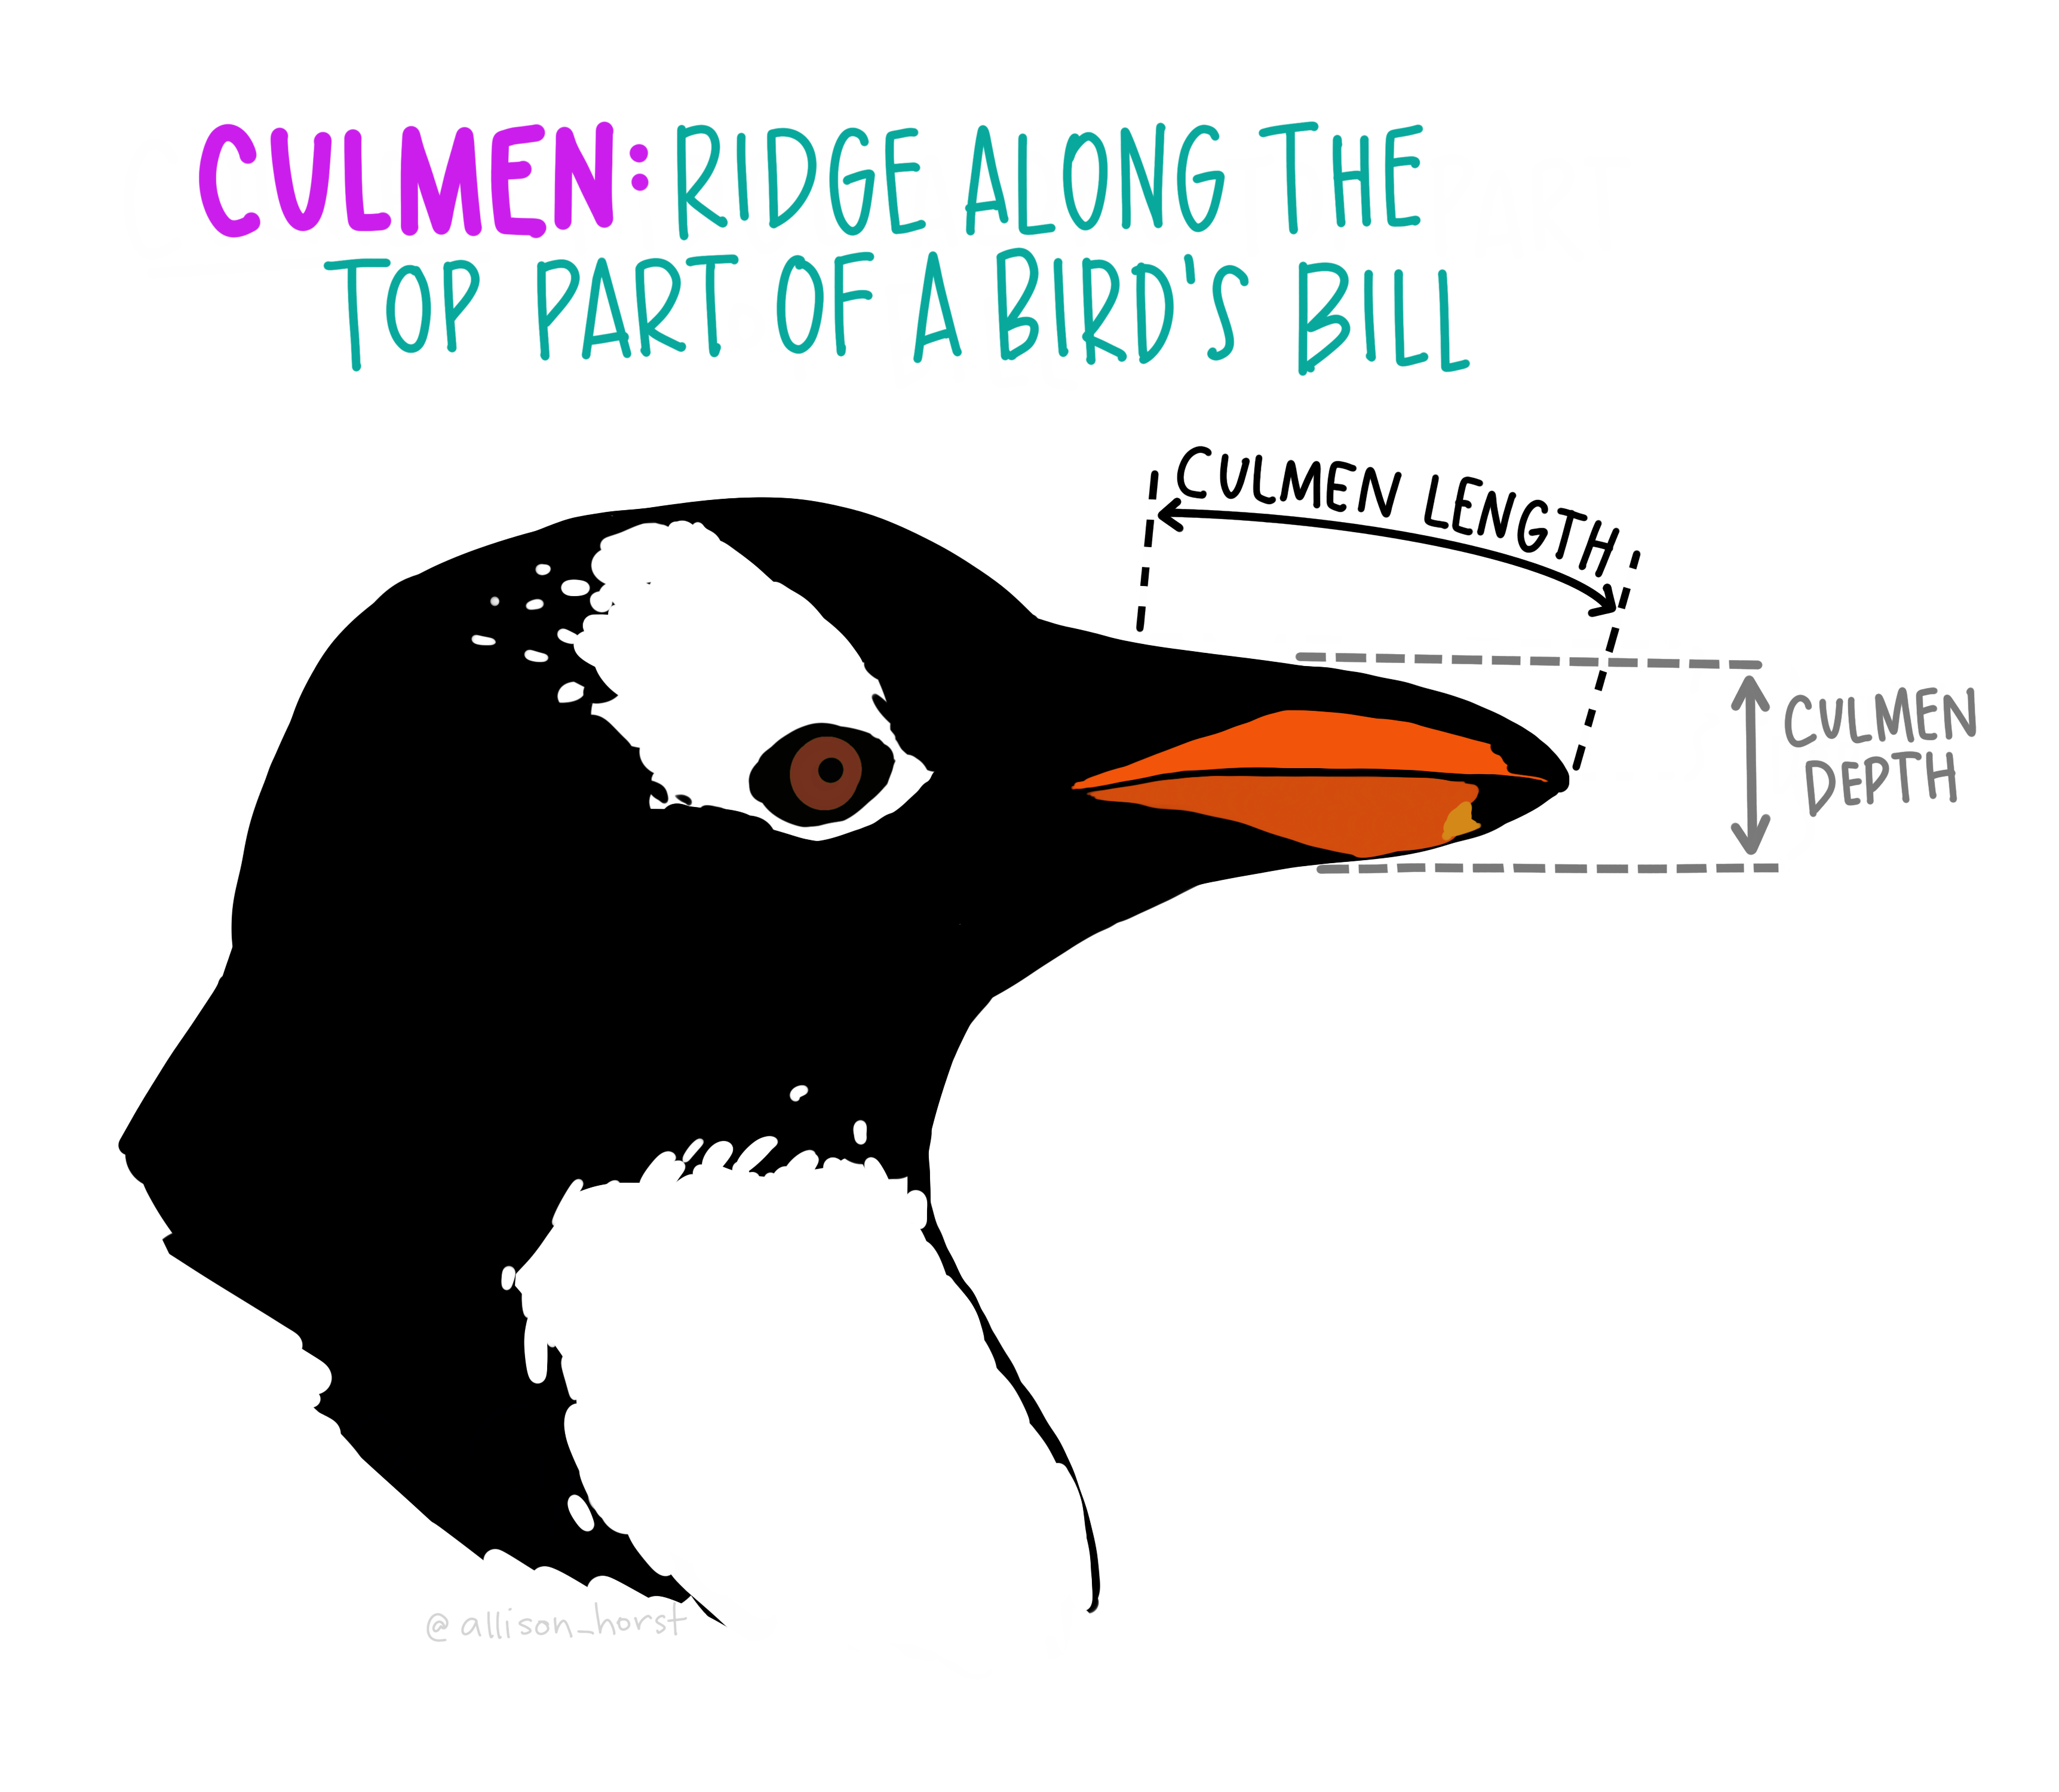
\includegraphics{culmen_depth}}, alto del culmen y la masa corporal de 342 pingüinos de las especies \emph{Pygoscelis adeliae} (Pingüino de Adelaida), \emph{Pygoscelis papua} (Pingüino Juanito), y \emph{Pygoscelis antarcticus} (Pingüino barbijo).

\begin{center}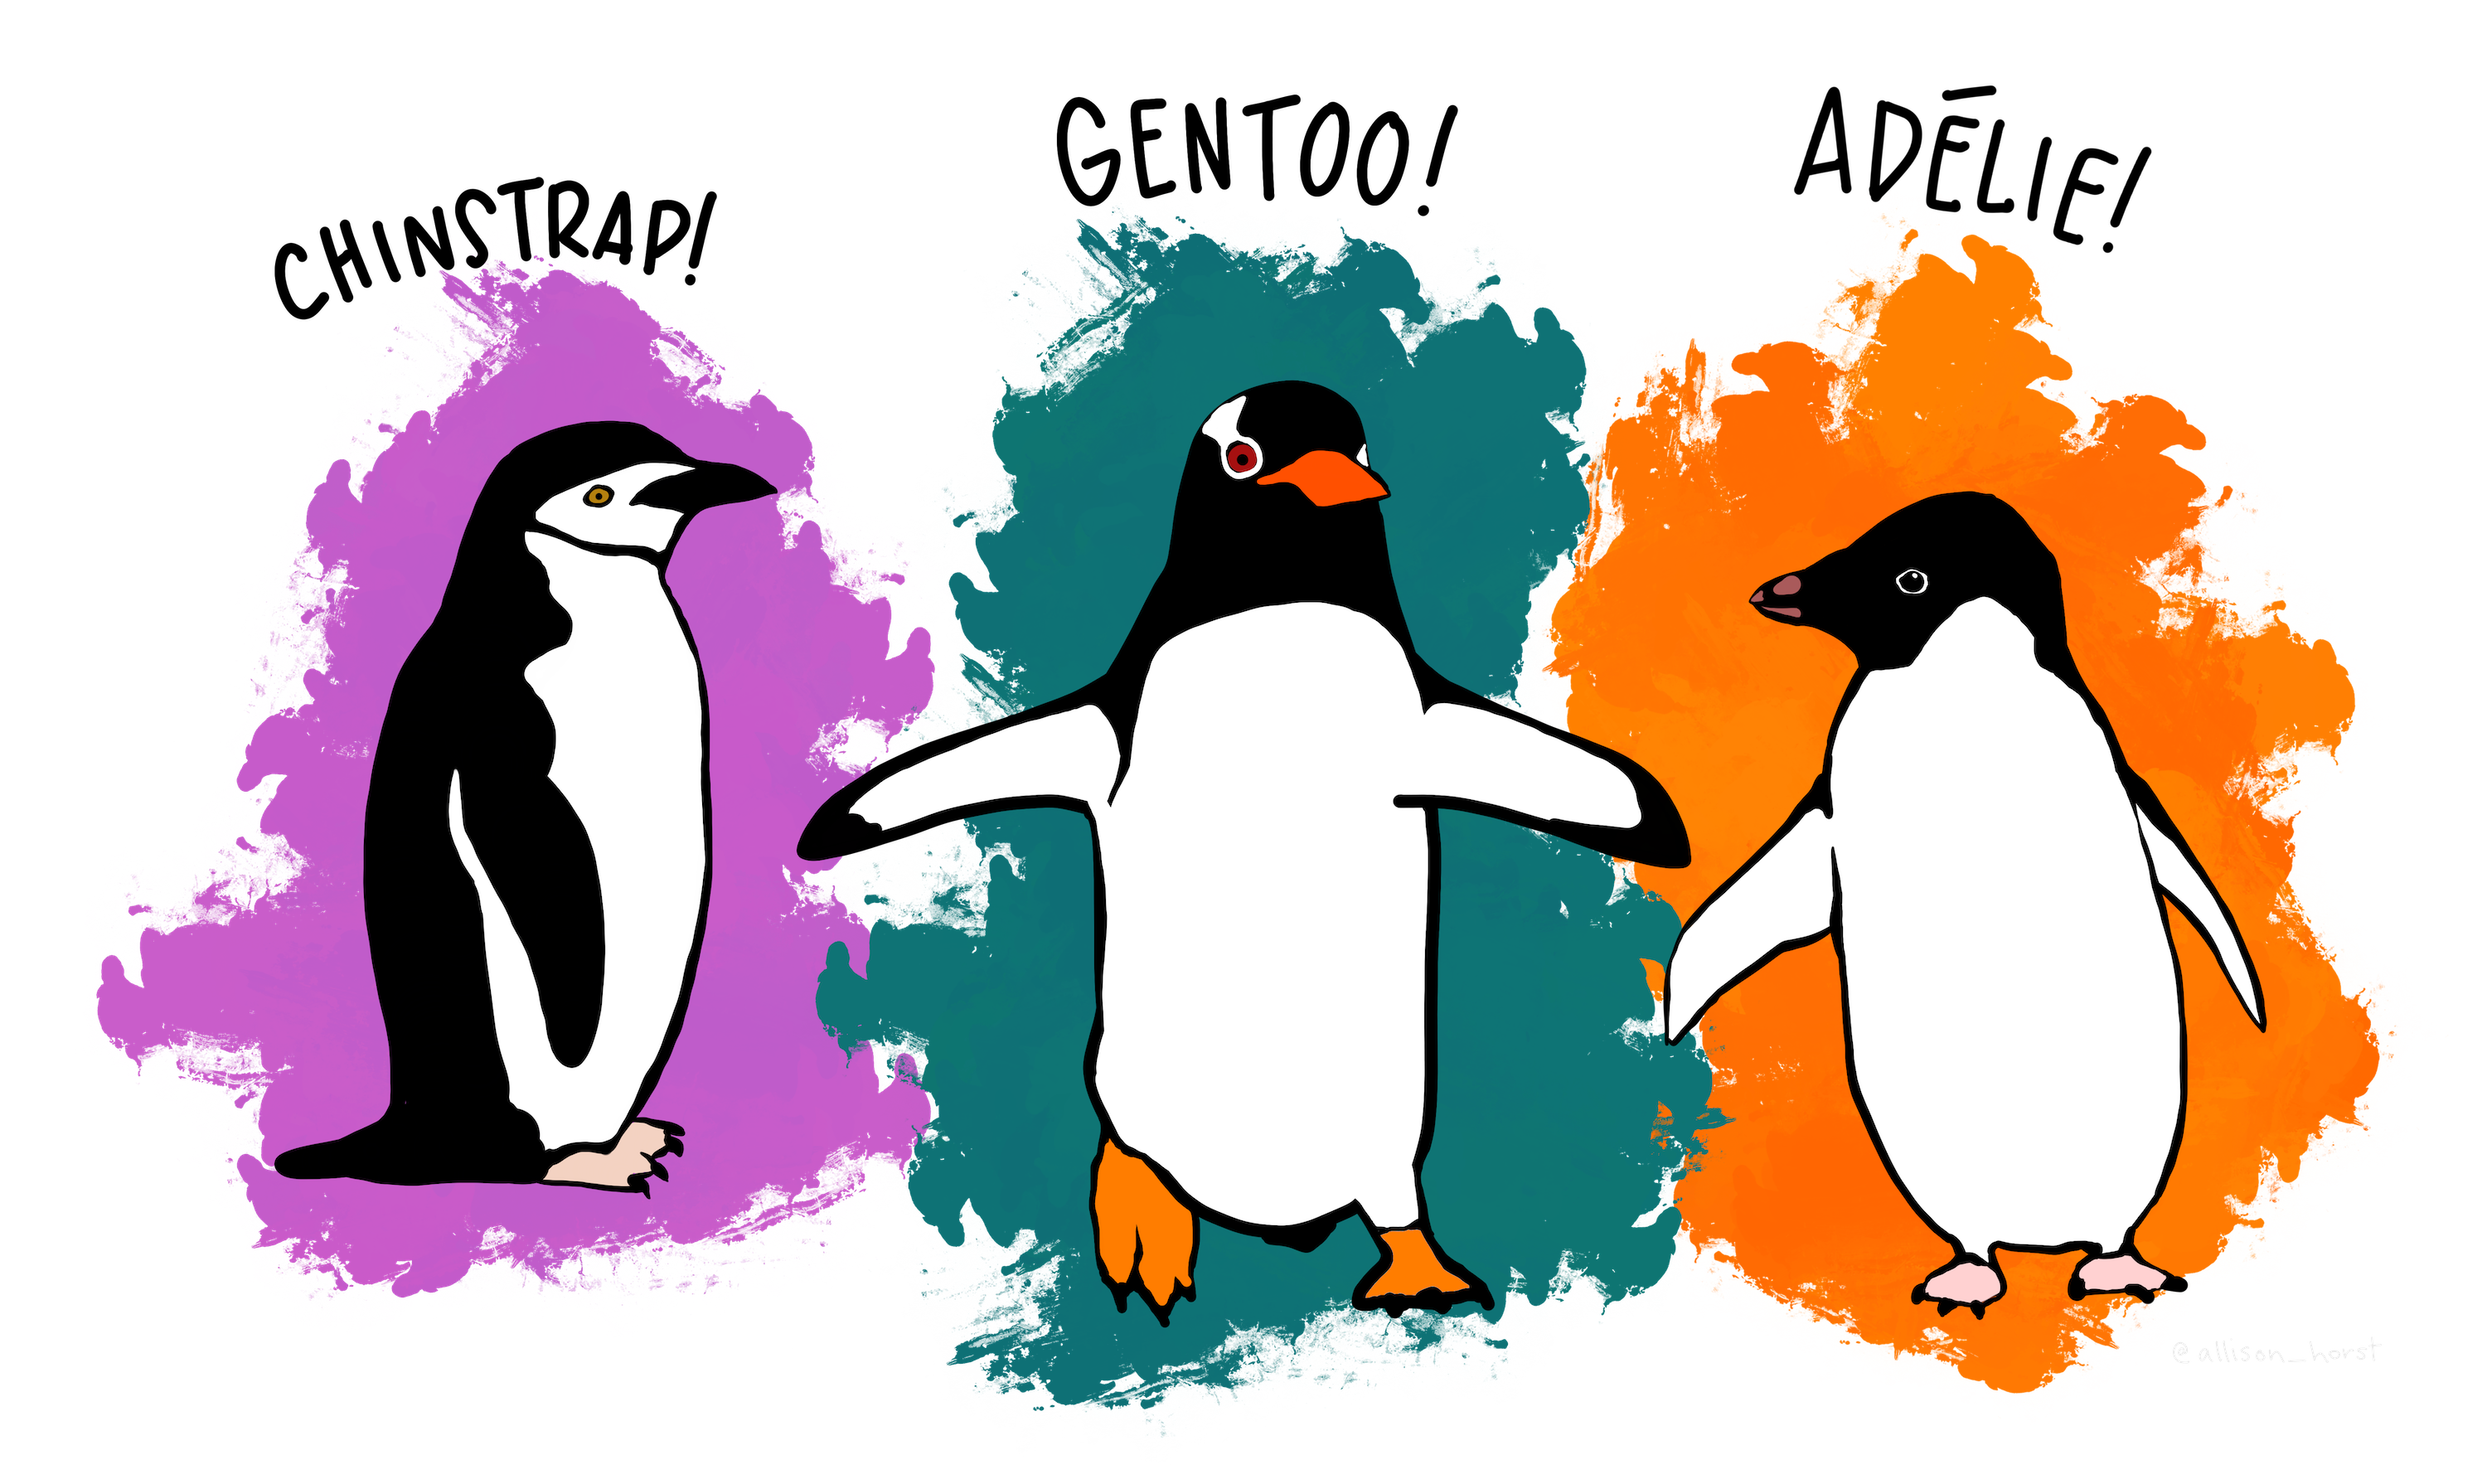
\includegraphics[width=0.8\linewidth]{penguins} \end{center}

En la Tabla \ref{tab:pen-glance} se muestran las primeras 3 mediciones para cada especie.

\begin{table}

\caption{\label{tab:pen-glance}Primeras 3 entradas de cada especie en los datos utilizados}
\centering
\begin{tabular}[t]{l>{\raggedleft\arraybackslash}p{2cm}>{\raggedleft\arraybackslash}p{2cm}>{\raggedleft\arraybackslash}p{2cm}>{\raggedleft\arraybackslash}p{2cm}}
\toprule
Especie & Longitud de culmen [mm] & Alto de culmen [mm] & Longitud de la aleta [mm] & Masa corporal [g]\\
\midrule
adelaida & 39.1 & 18.7 & 181 & 3750\\
adelaida & 39.5 & 17.4 & 186 & 3800\\
adelaida & 40.3 & 18.0 & 195 & 3250\\
juanito & 46.1 & 13.2 & 211 & 4500\\
juanito & 50.0 & 16.3 & 230 & 5700\\
\addlinespace
juanito & 48.7 & 14.1 & 210 & 4450\\
barbijo & 46.5 & 17.9 & 192 & 3500\\
barbijo & 50.0 & 19.5 & 196 & 3900\\
barbijo & 51.3 & 19.2 & 193 & 3650\\
\bottomrule
\end{tabular}
\end{table}

La variable categórica a predecir va a ser la especie, y las posibles variables predictoras son las dimensiones del culmen, la longitud de la aleta y la masa corporal. Es decir, en principio es un espacio de dimensión 4. Como la idea es trabajar en \(\mathbb{R}^2\), conviene explorar qué grado de separación permite cada combinación de dos variables. Esto se muestra en la Figura \ref{fig:pairs} donde se grafican scatterplots para todas las combinaciones de dos variables con la especie representada con color. Mirando las densidades de probabilidad (gráficos en la diagonal) se puede ver que la longitud del culmen separa bastante bien entre pingüino de adelaida y el resto mientras que las otras variables separan bien al pingüino juanito. Por lo tanto, las combinaciones que incluyen la longitud del culmen (gráficos en la primera columna) separan bastante bien entre las tres especies, mientras que el resto de las combinaciones tienen algún grado de mezcla entre pingüino de adelaida y pingüino juanito.

\begin{figure*}

{\centering 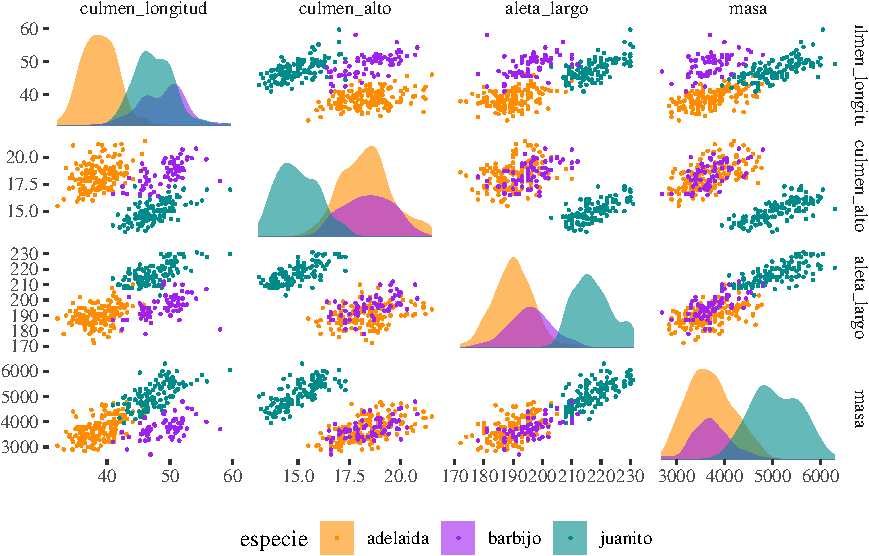
\includegraphics{TP-Labo-2_files/figure-latex/pairs-1} 

}

\caption[Scatteplot de todas las combinaciones de variables posibles en $\mathbb{R}^2$]{Scatteplot de todas las combinaciones de variables posibles en $\mathbb{R}^2$. En la diagonal, estimaciones de densidad de cada variable separadas por especies.}\label{fig:pairs}
\end{figure*}

En lo que sigue, voy a usar los datos de Longitud de culmen y de alto del culmen para separar entre las tres especies.

\hypertarget{clasificador-cuadruxe1tico}{%
\section{Clasificador cuadrático}\label{clasificador-cuadruxe1tico}}

\begin{center}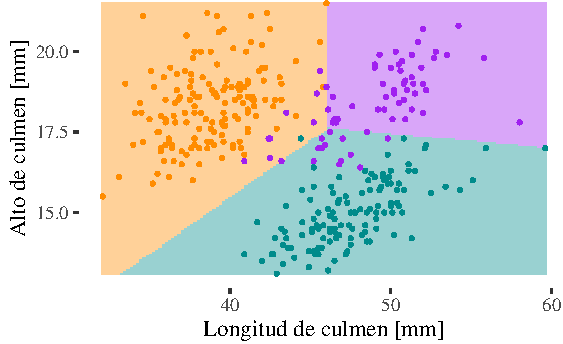
\includegraphics{TP-Labo-2_files/figure-latex/unnamed-chunk-6-1} \end{center}

\begin{center}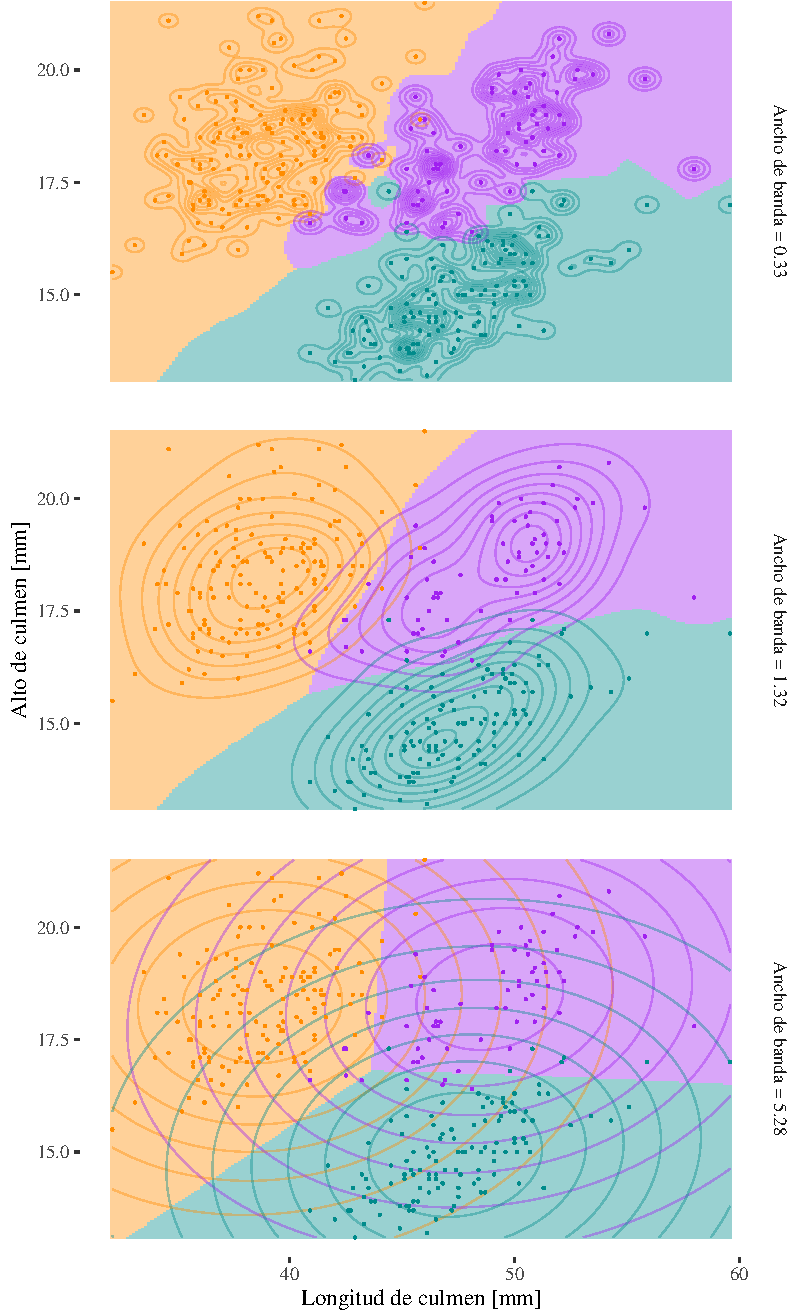
\includegraphics{TP-Labo-2_files/figure-latex/unnamed-chunk-7-1} \end{center}

\hypertarget{fisher}{%
\subsection{Fisher}\label{fisher}}

\begin{center}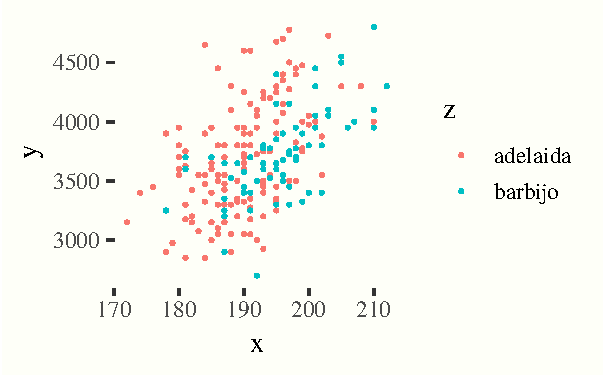
\includegraphics{TP-Labo-2_files/figure-latex/unnamed-chunk-11-1} \end{center}

\begin{center}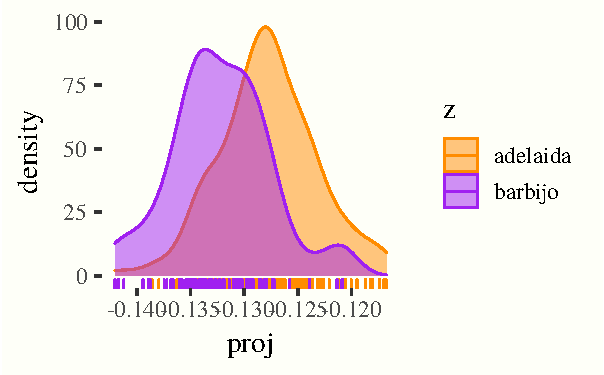
\includegraphics{TP-Labo-2_files/figure-latex/unnamed-chunk-11-2} \end{center}

\hypertarget{loguxedstica}{%
\subsection{Logística}\label{loguxedstica}}

\begin{center}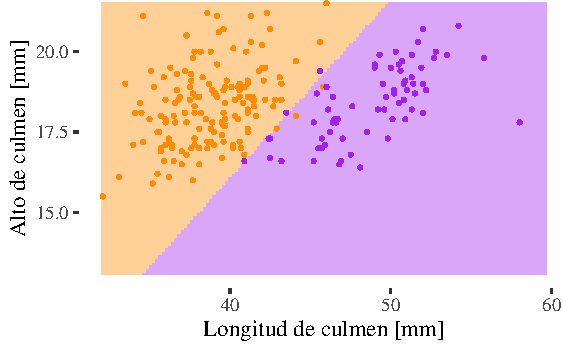
\includegraphics{TP-Labo-2_files/figure-latex/unnamed-chunk-12-1} \end{center}

\hypertarget{referencias}{%
\section*{Referencias}\label{referencias}}
\addcontentsline{toc}{section}{Referencias}

\hypertarget{refs}{}
\leavevmode\hypertarget{ref-R-palmerpenguins}{}%
KB, Gorman, Williams TD, and Fraser WR. 2014. ``Ecological Sexual Dimorphism and Environmental Variability Within a Community of Antarctic Penguins (Genus Pygoscelis).'' \emph{PLoS ONE} 9(3) (e90081): --13. \url{https://doi.org/10.1371/journal.pone.0090081}.



\end{document}
